\hoofdstuk{Case study}
\paragraaf{Introduction}
This chapter introduces iStager and summarizes its development process. iStager is be a cross-platform mobile application developed using Titanium. The summary will cover the application requirements and design, the implementation process and the results. 


% The implementation consists of feature availability of Titanium, and the possible augmentation of missing features.  

%As mentioned in the chapter \emph{Main research} the goal is to answer the question: "\emph{Is Titanium viable for commerical useage?}" 
% To answer this question a set of criteria have been defined in the chapter \emph{Main research}, section \emph{Defining viable}


% \begin{itemize}
% 	\item \emph{Extensibility}
% 	\item \emph{Maturity}
% 	\item \emph{Documentation}
% \end{itemize}

\paragraaf{Stager}
In 2011, live music venue WORM hired Lunatech to build \emph{Stager}, a modern web-based resource planning and ticketing application to help manage live music events. Lunatech took the opportunity to use the relatively new Play framework to build a web application with an HTML5 and Java architecture. Stager has broad requirements ranging from high performance and security for the public ticket sales component to high usability for the internal resource planning component that will be used for hours a day by employees and being open to enhancements in the future for new customers. \cite{Lunatech2011} In April 2012 Stager became Stager B.V. and is able to function independently from WORM. As main marketing concept Stager B.V. offers the use of Stager  to live music venues. Although WORM is the main customer of Stager B.V. this might change in the future as Stagers market share expands. 

\subparagraaf{WORM}
WORM is an institute for avantgardistic recreation Rotterdam, consisting of an artistscollective, a podium with a bar and Parallel University (DIY workshops for film, music and media). Born under the stars of punk, Dada, Fluxus, Situationism and futurism WORM is grown into a headstrong organization that the 'Do-It-Yourself' mentality of their ancestors, combined with ultra-pragmatism, love of technique (s) and proper accounting. Worm outputs film, radio, concerts, courses, parties, publications, performances, web projects, installations, workshops and an accumulation of tactile media and internet.WORM focuses (cheerful yet serious) in avantgarde, resource scarcity and open source. \cite{WORM2012} Due to a drain on subsidized funding resource from the government WORM is forced halt its' current operations. It is possible that WORM closes its doors in august 2012, alternatively WORM might reorganize and continue in a s smaller form.

\paragraaf{Introducing iStager}
iStager is a mobile event publication platform. As described above Stager is an planning and ticketing application to help manage live music events. In addition to planning and ticketing Stager features an \emph{atomfeed} to publish events. iStager makes use of this atom-feed to publish planned events on a mobile device. Because Stager
Every customer of Stager would be granted their own version of iStager. This indicates that iStager needs to be have a generic user interface.


\paragraaf{Stager application requirements}

%todo: tussen delen naar appendix. 
Functional requirements:
\begin{enumerate}
\item \emph{Cross-platform}\\Application must be compatible to run on iOS 4.3 or greater \emph{and} Android 2.2 or greater.
\item \emph{Native look-and-feel}\\Application must make use the of the native user interface components.
\item \emph{i18n}\\Application must have language support for both Dutch and English.
\item \emph{Generic style}\\Application must have an configurable stylesheet to generate different styles of user interface looks.
\end{enumerate}

\noindent Below is a simplified list of the feature requirements of the iStager application.\footnote{The complete set of requirements is attached as an appendix} %TODO apendix.
\begin{enumerate}
\item
List of current and upcoming events
\item
Detail-view of an event, shows detailed event information of an selected event:
\item
Add event to agenda
\item
Start GPS-based navigation towards physical location of event
\item
View media attached to an event
\item
Display in a grid or list, categorize media types.
\item
Share event details to social media
% \item
% (Un)Register device to receive push notifications on new events of interest
% \item
% Register the device to receive pushed notifications about upcoming events which might be of interest to the user.
% Based on Relation.interest model in Stager.
\end{enumerate}

\paragraaf{Architecture}
The global architecture consists of a client-server model where the mobile application acts as the client, and the Stager application provides acts as the server.

\begin{centering}
	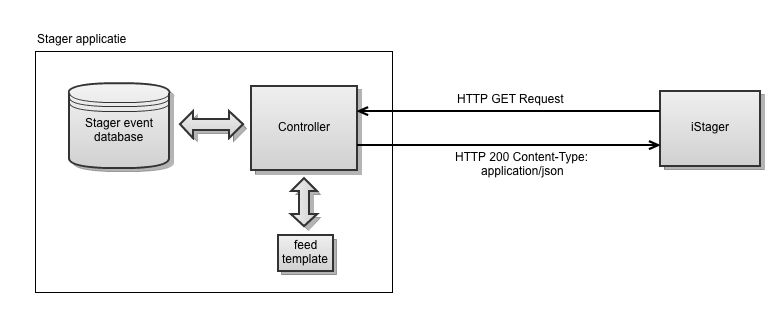
\includegraphics[scale=0.4]{images/globale_architectuur.png}\\{The client-server architecture of Stager and the iStager app}\\
\end{centering}

\paragraaf{Design}
The application designed in consultation with WORM. It had to be modern enough to stand out from other apps, yet it had to simple enough to support an generic stylesheet.


\subparagraaf{User interaction}
\begin{centering}
	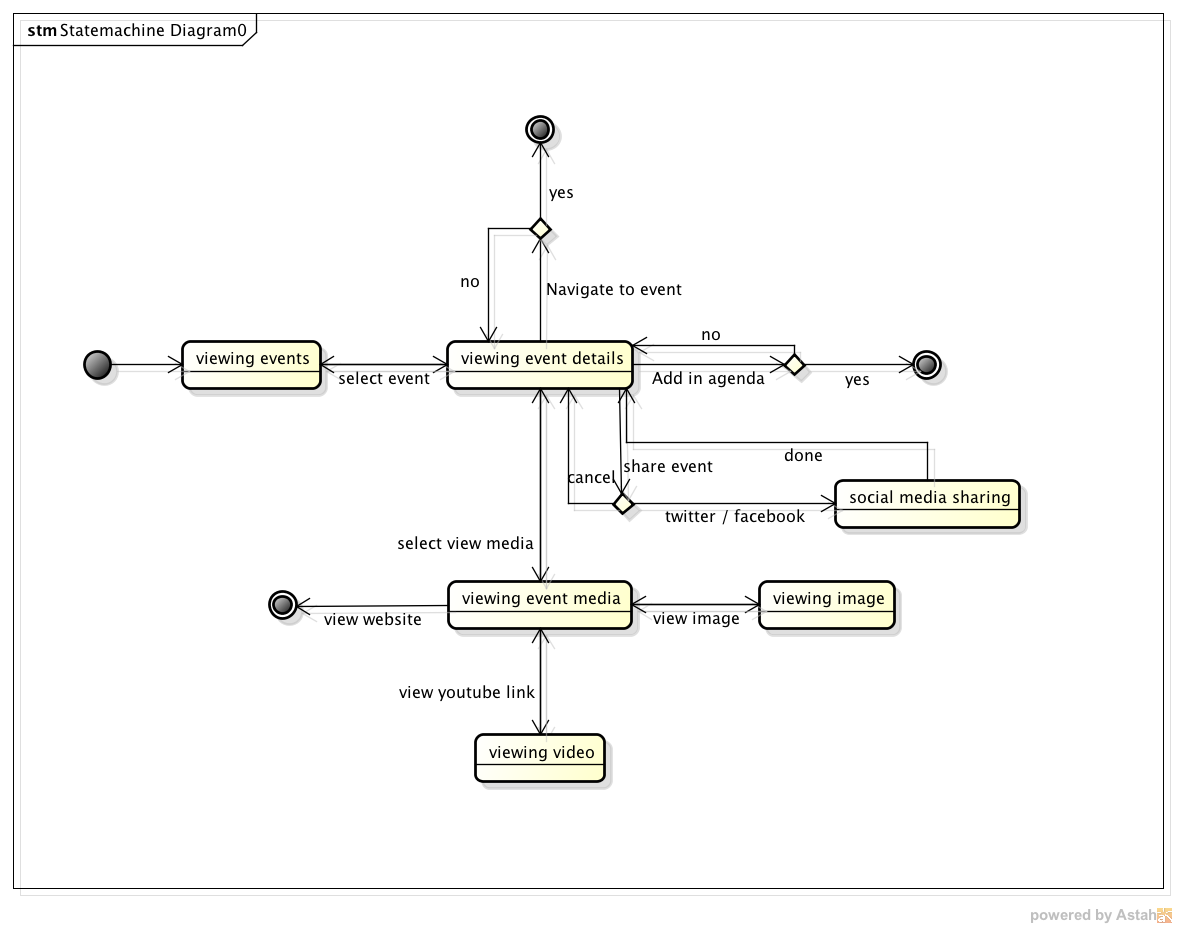
\includegraphics[scale=0.4]{images/stagerapp_statediagram.png}\\{Flowchart diagram of the iStager app}\\
\end{centering}


\paragraaf{Feed}
Stager is able to publish any planned live music events trough an feed which is publicly accessible. An feed is an simplified standardized view of content which may be frequently updated. In Stager the feed has an atom-based XML format.

\paragraaf{Events}
An event contains contains detailed information about an occurrence at a certain time, date and location. The detailed information consists of a title, subtitle, content, attached media. 

\paragraaf{Media}
When an event is gets published it is possible to attach media items to the publication. These range from audio files and images to  links to websites such as to youtube content. Any attached media will be included in the feed as a hyperlink to its location, which is publicly accessible.

\paragraaf{i18n}


\paragraaf{Issues}

An issue was the lack of DOM3 specification support. This was already determined during the development of the benchmark application in the preliminary research, however the chosen solution was a quick fix to solve the symptom of the issue. 

\paragraaf{Results}


% \subparagraaf{Platform support}
% \subparagraaf{Native look and feel}

\begin{figure}%
	\centering
	\parbox{0.0in}
	\qquad
	\begin{minipage}{2.2in}%
		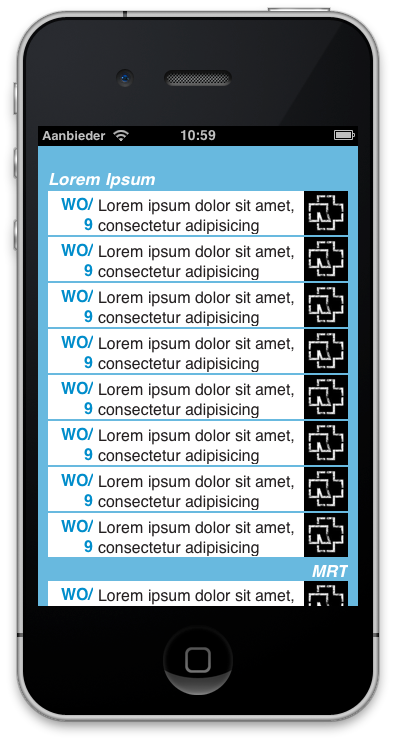
\includegraphics[scale=0.15]{images/iStager_1.png}
		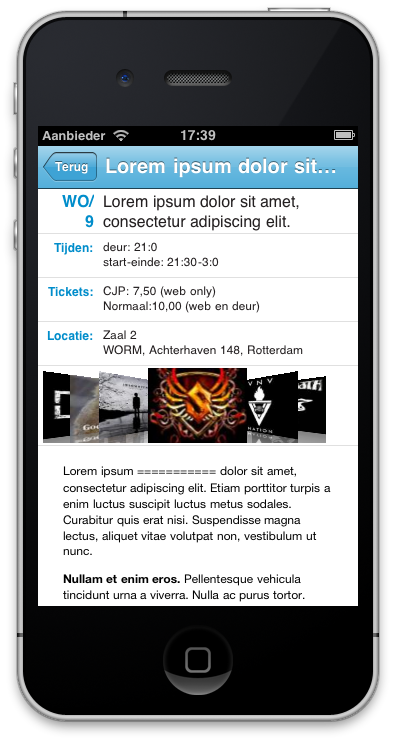
\includegraphics[scale=0.15]{images/iStager_2.png}
	\end{minipage}%
	\caption{iStager application on running iOS 5.0}%
	\label{fig:1figs}%
\end{figure}
\subparagraaf{DOM2 issue}
%feed -> json.
\subparagraaf{Tableview performance}

\subparagraaf{Cross-platform NavigationController}


\paragraaf{Conclusion}
%Samenvatten wat er gedaan is aan de Stager app, welke platforms het draaid, e.d.
Although not completely finished due to time restrains, the development of iStager proved that it is possible to build a cross-platform application which is truly native.

